\subsection{Understanding SDR Receiver Overload Levels!}

\begin{tcolorbox}[colback=gray!10, colframe=black, title=E4C08`]
An SDR receiver is overloaded when input signals exceed what level? 

\begin{enumerate}[label=\Alph*.]
    \item One-half of the maximum sample rate
    \item One-half of the maximum sampling buffer size
    \item The maximum count value of the analog-to-digital converter
    \item \textbf{The reference voltage of the analog-to-digital converter}
\end{enumerate} \end{tcolorbox}

\subsubsection{Concepts Related to SDR Overload Levels}

To understand the overload levels of a Software Defined Radio (SDR) receiver, it's essential to grasp the role of the analog-to-digital converter (ADC) within the receiver system. The ADC is a crucial component that converts analog signals into digital signals for further processing. 

When discussing SDR performance, the reference voltage of the ADC sets the maximum allowable input level before distortion occurs. If the input signal exceeds this reference voltage, the ADC cannot accurately convert the input signal into digital data, leading to what is known as overload.

\subsubsection{Understanding ADC Overload}

An SDR receiver experiences overload at input signal levels exceeding the reference voltage of its ADC. This concept can be mathematically represented as:

\[
\text{Overload Condition: } V_{\text{input}} > V_{\text{ref}}
\]

where:
- \( V_{\text{input}} \) is the input signal voltage.
- \( V_{\text{ref}} \) is the reference voltage of the ADC.

Let's denote the maximum count value of an ADC as:

\[
V_{\text{max}} = V_{\text{ref}} \times \text{Resolution}
\]

The resolution of an ADC (in bits) determines how finely it can distinguish between different voltage levels. For example, a 12-bit ADC has a resolution of \( 2^{12} = 4096 \).

\subsubsection{Conclusion}

Hence, for an SDR receiver, it is critical to ensure that the input signals do not exceed the reference voltage of the ADC. Monitoring and limiting the input signal amplitude can prevent overload conditions, which can lead to signal distortion and loss of information.

\begin{center}
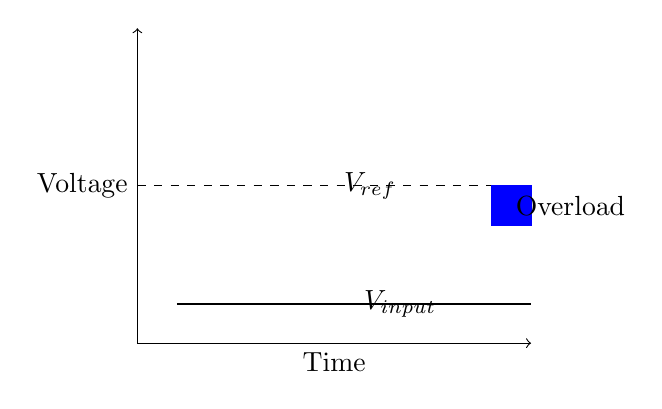
\begin{tikzpicture}
    \draw[->] (0,0) -- (5,0) node[midway, below] {Time};
    \draw[->] (0,0) -- (0,4) node[midway, left] {Voltage};
    \draw[thick] (0.5,0.5) -- (5,0.5) node[midway, right] {$V_{\text{input}}$};
    \draw[dashed] (0,2) -- (5,2) node[midway, right] {$V_{\text{ref}}$};
    \filldraw[blue] (4.5,1.5) rectangle (5,2);
    \node at (5.5,1.75) {Overload};
\end{tikzpicture}
\end{center}
